% !TEX root = ../../I4PRJ, Grp3 - Rapport.tex


\subsubsection{\gls{mu}}
En \gls{mu} registreres hos \gls{smartpool} gennem \gls{pcapp} applikationen. Med hver \gls{mu} medfølger et serienummer som bruges ved registrering. En \gls{mu} er enheden der måler pH, frit\footnote{Frit klor angriber bakterier, alger og svampeorganismer. Med tiden transformeres frit klor til bunden klor.}\todo{Find reference eller fjern sætning.} klor og total\footnote{Total klor er summen af frit klor og bunden klor.} klor samt varmeværdier i en \gls{pool}. Det er \gls{mu} der står for behandling af rå. Da der er en sammenhæng figur~\ref{fig:chlorinePh} mellem målte pH-værdier og effektivitet af frit klor\todo{reference!} skal den rå data gennemgå en hidtil udefineret matematisk behandling for at kunne vise \gls{user} relevant information. De rå data bruges til at beregne forholdet mellem bunden klor, som er ineffektivt, lugter kraftigt og irriterer øjne\todo{Referencer!} og slimhinder, og frit klor samt \glspl{pool} overordnede sundhedskarakteristika. \gls{mu} ansvar er således:

\paragraph{Måling af data}
\begin{itemize}
	\item Måling af total klor.
	\item Måling frit klor.
	\item Måling af pH-værdi.
	\item Måling af Temperatur.
\end{itemize}

\paragraph{Behandling af rå data}
\begin{itemize}
	\item Beregning af bunden klor.
	\item Beregning af klor der bør tilføres/fjernes fra \gls{pool}.
	\item Beregning af den mængde syre/base der skal tilføres \gls{pool}.
\end{itemize}

\begin{figure}
	\centering
	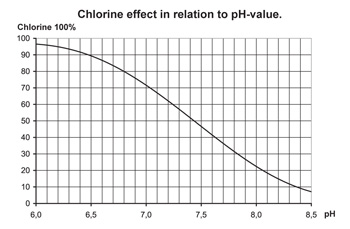
\includegraphics[width=0.7\linewidth]{figs/chlorinePh.png}
	\caption{Sammenhæng mellem effektivitet af frit klor og pH værdi. Kilde: \url{http://www.pahlen.com/users-guide/ph-and-chlorine}}
	\label{fig:chlorinePh}
\end{figure}


\subsubsection{\gls{pool}}
Pool er den enhed der males på. En Pool kan være af hvilken som helst størrelse og form. Hver Pool kan associeres med en \gls{mu}.